\subsection{Overall accuracy of Simplified Ikeda method}
\label{se:overall_comparison}
An investigation of how well the implementation of the simplified Ikeda's method (see section \ref{se:semi-empirical methods}) agree with the corresponding results in the roll damping database has been carried out. 

Comparing roll damping is a bit difficult since the roll damping model consist of two coefficients, a linear term $B_1$ and a quadratic term $B_2$. These coefficients can be combined by calculating the equivalent damping coefficient for a certain roll angle $\phi_a$ \parencite{himeno_prediction_1981}:

\begin{equation}
B_{e} = B_{1} + \frac{8 B_{2} \omega_{0} \phi_{a}}{3 \pi}
\end{equation}

where $\phi_a$ was taken as the initial/maximum roll angle from the roll decay tests. It is also a measure to describe the nonlinear properties of a ship's roll damping from the tests. For the roll damping database $B_1$ and $B_2$ can be inserted directly into the Eq. (\ref{eq:B_e_equation}) to get the equivalent roll damping $B_e$.

In order to obtain the same coefficients for the simplified Ikeda's method, roll damping was calculated for two or more roll amplitudes $\phi_a$ for the same motion frequency. $B_1$ and $B_2$ are obtained by fitting the Eq. (\ref{eq:B_e_equation}) to this data. The $B_e$ coefficient was made non-dimensional according to \parencite{himeno_prediction_1981}  giving the non-dimensional equivalent linear damping coefficient $\hat{B_e}$, which was more convenient to use for this comparison as follows,
\begin{equation} \label{eq:be_eqvalent}
    \hat{B_e} = \frac{B_e}{\rho \bigtriangledown Beam^2} \sqrt{\frac{Beam}{2g}}
\end{equation}
where $\rho$, $\bigtriangledown$ and $Beam$ stand for fluid density, displacement volume and breadth of a ship, respectively.


For the roll decay tests at SSPA, i.e., the database used in this study, the initial roll angle is normally set to 10 degrees. In order to have a fair comparison with the simplified Ikeda's method (SI-method), the motion response signal from the SSPA tests are truncated such that the initial roll angels $\phi_a$ equal to various initial roll degrees. Then, the roll damping coefficients for these truncated motion signals can be estimated. The coefficient of determination $R^2$ of the equivalent roll damping for various initial roll angles $\hat{B}_e(\phi_a)$ between estimation by the simplified Ikeda's method and the model test results is plotted in the upper plot of Fig.\ref{fig:ikeda_phi_a}. The low values of $R^2$ indicate very bad agreement between the simplified Ikeda's method and the model test results for roll damping prediction of modern ships. It should be noted that the accuracy decrease for larger amplitudes where nonlinear part of the SI-method plays a larger part. Furthermore, in order to illustrate the difference of $\hat{B}_e$ prediction between the SI-method and the model tests at SSPA, the three bottom plots of Fig.\ref{fig:ikeda_phi_a} presents the comparison for three roll amplitudes $\phi_a$ equal to 0, 5, 10 degrees, respectively. It shows that the accuracy differ very much between the amplitudes, with the highest accuracy at zero roll amplitude. 


\begin{figure}[H]
\centering
  \centering
  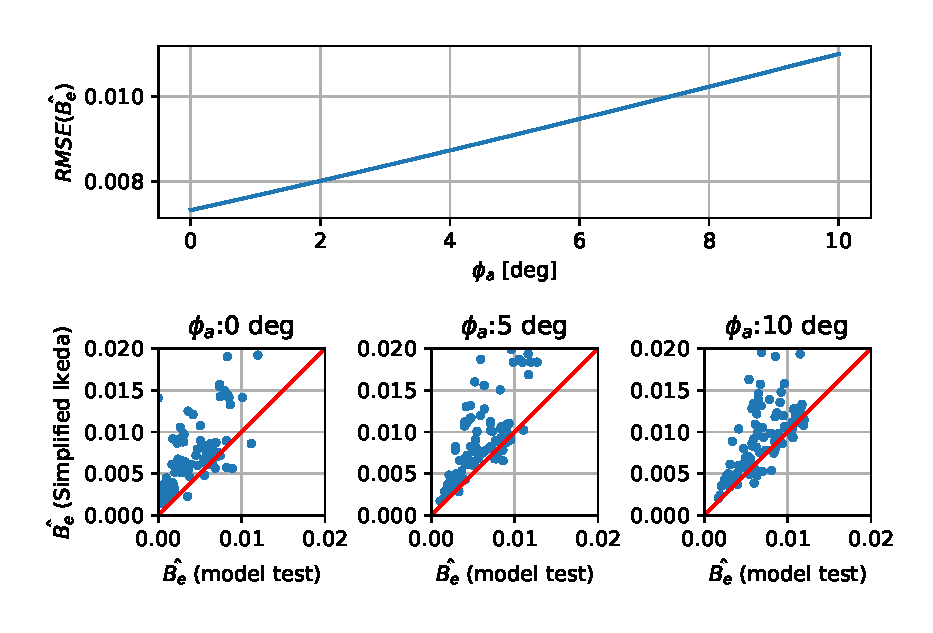
\includegraphics[]{figures/ikeda_phi_a.eps}
  \vspace{-0.5cm}
  \caption{Root mean square error of roll damping prediction between the SI-method and the model test results (upper plot). Influence of roll amplitude $\phi_a$ on $\hat{B_e}$ between the SI-method and model tests for $0^{\circ}$ (bottom left plot), $5^{\circ}$ (bottom middle plot) and $10^{\circ}$ (bottom right plot), respectively.}
  \label{fig:ikeda_phi_a}
\end{figure}

To use the whole motion signals from the roll decay tests for the prediction of roll damping, it was however found that a smaller value of 2 degrees gave better agreement and was instead used in the following analysis. 
It was found that almost all ships in the roll damping database were outside the limits that are suitable to be applied in Eq.(\ref{eq:SI_limits}). Two different ways to handle this limit exceedance was investigated:
\begin{enumerate}
  \item the ``unlimited" approach where the input values are allowed to exceed the limits.
  \item the ``limited" approach where the limit boundary values were used for exceeding values.
\end{enumerate}

Figure \ref{fig:ikeda_limited} show the comparison of roll damping predictions by the Simplified Ikeda's method using the ``unlimited" and ``limited" approach with the corresponding results from model tests. The ``limited" approach seems to be the best one to use according to this figure, where the ``unlimited" approach has values very far away from the model test results (as the red reference line).   
The large deviations with the ``unlimited" approach seem to originate from the wave damping coefficient $\hat{B_W}$ according to Fig. \ref{fig:ikeda_components}. Also the bilge keel damping coefficient $\hat{B_{BK}}$ seems to suffer from extrapolation when the ``unlimited" approach is used. 

\begin{figure}[H]
\vspace{-0.5cm}
\centering
  \centering
  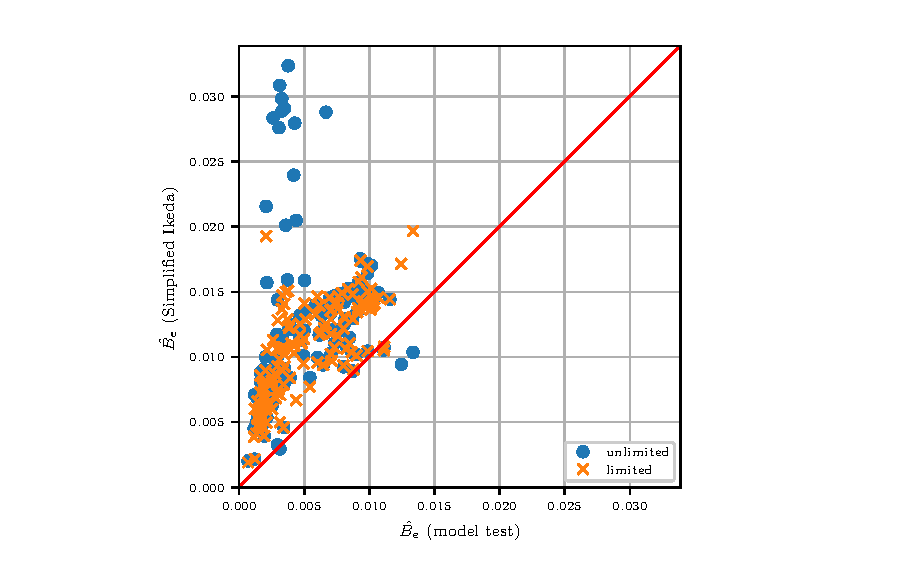
\includegraphics[height=5cm, width = 10cm]{figures/ikeda_limited.eps}
  \vspace{-0.5cm}
  \caption{$\hat{B_e}$ at all speeds estimated by the simplified Ikeda's method (Y-axis) in comparison with that from the roll decay test database (X-axis)}
  \label{fig:ikeda_limited}
\end{figure}


\begin{figure}[H]
\vspace{-0.5cm}
\centering
  \centering
  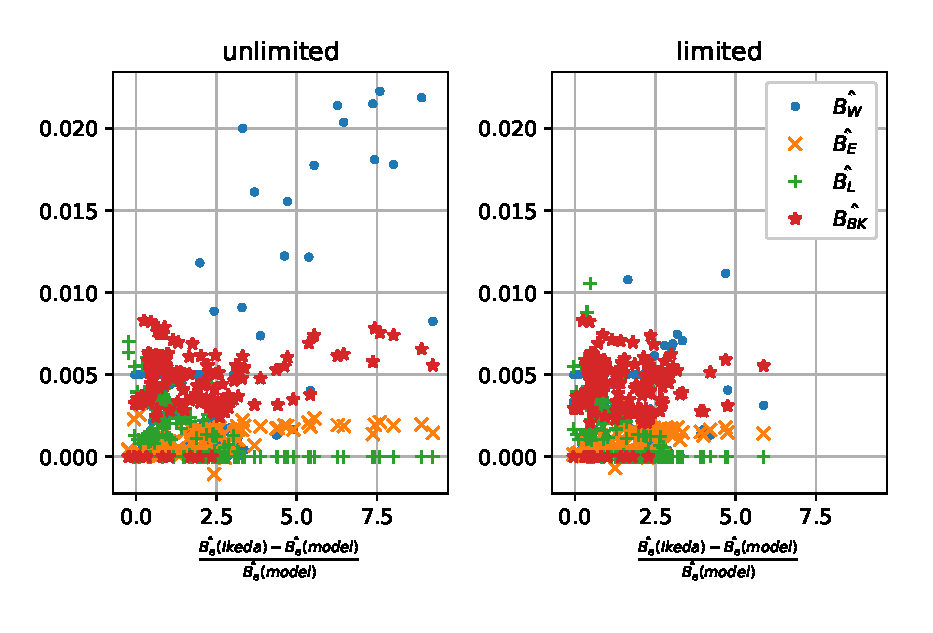
\includegraphics[height=6cm, width = 14cm]{figures/ikeda_components.eps}
  \vspace{-0.5cm}
  \caption{Investigation of how the roll damping components influence the error for the ``unlimited" and ``limited" approach to input extrapolation}
  \label{fig:ikeda_components}
\end{figure}

\textbf{\textit{Remarks:}} From the above analysis, it is found that the simplified Ikeda's method was built based on very old ships, while the dimensions of modern ships are mostly beyond the limits that can be applied by Ikeda's method. This makes the prediction by the simplified Ikeda's method differ significantly from the model test results.
Therefore, it is an urgent task to propose either a complete new method to replace Ikeda's method, or make corrections to the Simplified method to be able to accurate predict a modern ship's roll damping coefficients. A preliminary attempt will be tested in the following section based on the SSPA model test database.